\chapter{The Social AR Continuum} % Main chapter title
\label{ch:continuum} % Change X to a consecutive number; for referencing this chapter elsewhere, use \ref{ChapterX}

This chapter describes The Social AR Continuum, a space that encompasses different dimensions of Augmented Reality (AR) for sharing social experiences. We explore various dimensions, discuss options for each dimension, and outline possible scenarios where these options might be useful. We categorise the social AR dimensions into three areas: 1) Self and others, 2) Surrounding environment, and 3) Interactions.

Representing self and others as avatars is described in more detail in Chapter \ref{ch:contacts}. The surrounding environment and sharing different types of data is described in more detail in Chapter \ref{ch:data}, while the interactions between people in form of annotation on the surrounding environment is described in Chapter \ref{ch:annotation}.

% \section{Concept}
% \section{General System Implementation}
% \section{Evaluation}

% =============== PREVIOUS WORK ================
% A. Nassani, G. Lee, M. Billinghurst, T. Langlotz, S. Hoermann and R. W. Lindeman, “[Poster] The Social AR Continuum: Concept and User Study” in ISMAR 2017
% =============== PREVIOUS WORK ================

% \section{Abstract}
% \label{sec:continuum-abstract}

In this work, we describe The Social AR Continuum, a space that encompasses different dimensions of Augmented Reality (AR) for sharing social experiences. We explore various dimensions, discuss options for each dimension, and explore possible scenarios where these options might be useful. We describe a prototype interface using the \textit{contact placement} dimension, and report on feedback from potential users which supports its usefulness for visualising social contacts. Based on this concept work, we suggest user studies in the social AR space, and give insights into future directions. 

\begin{figure}
    \centering
    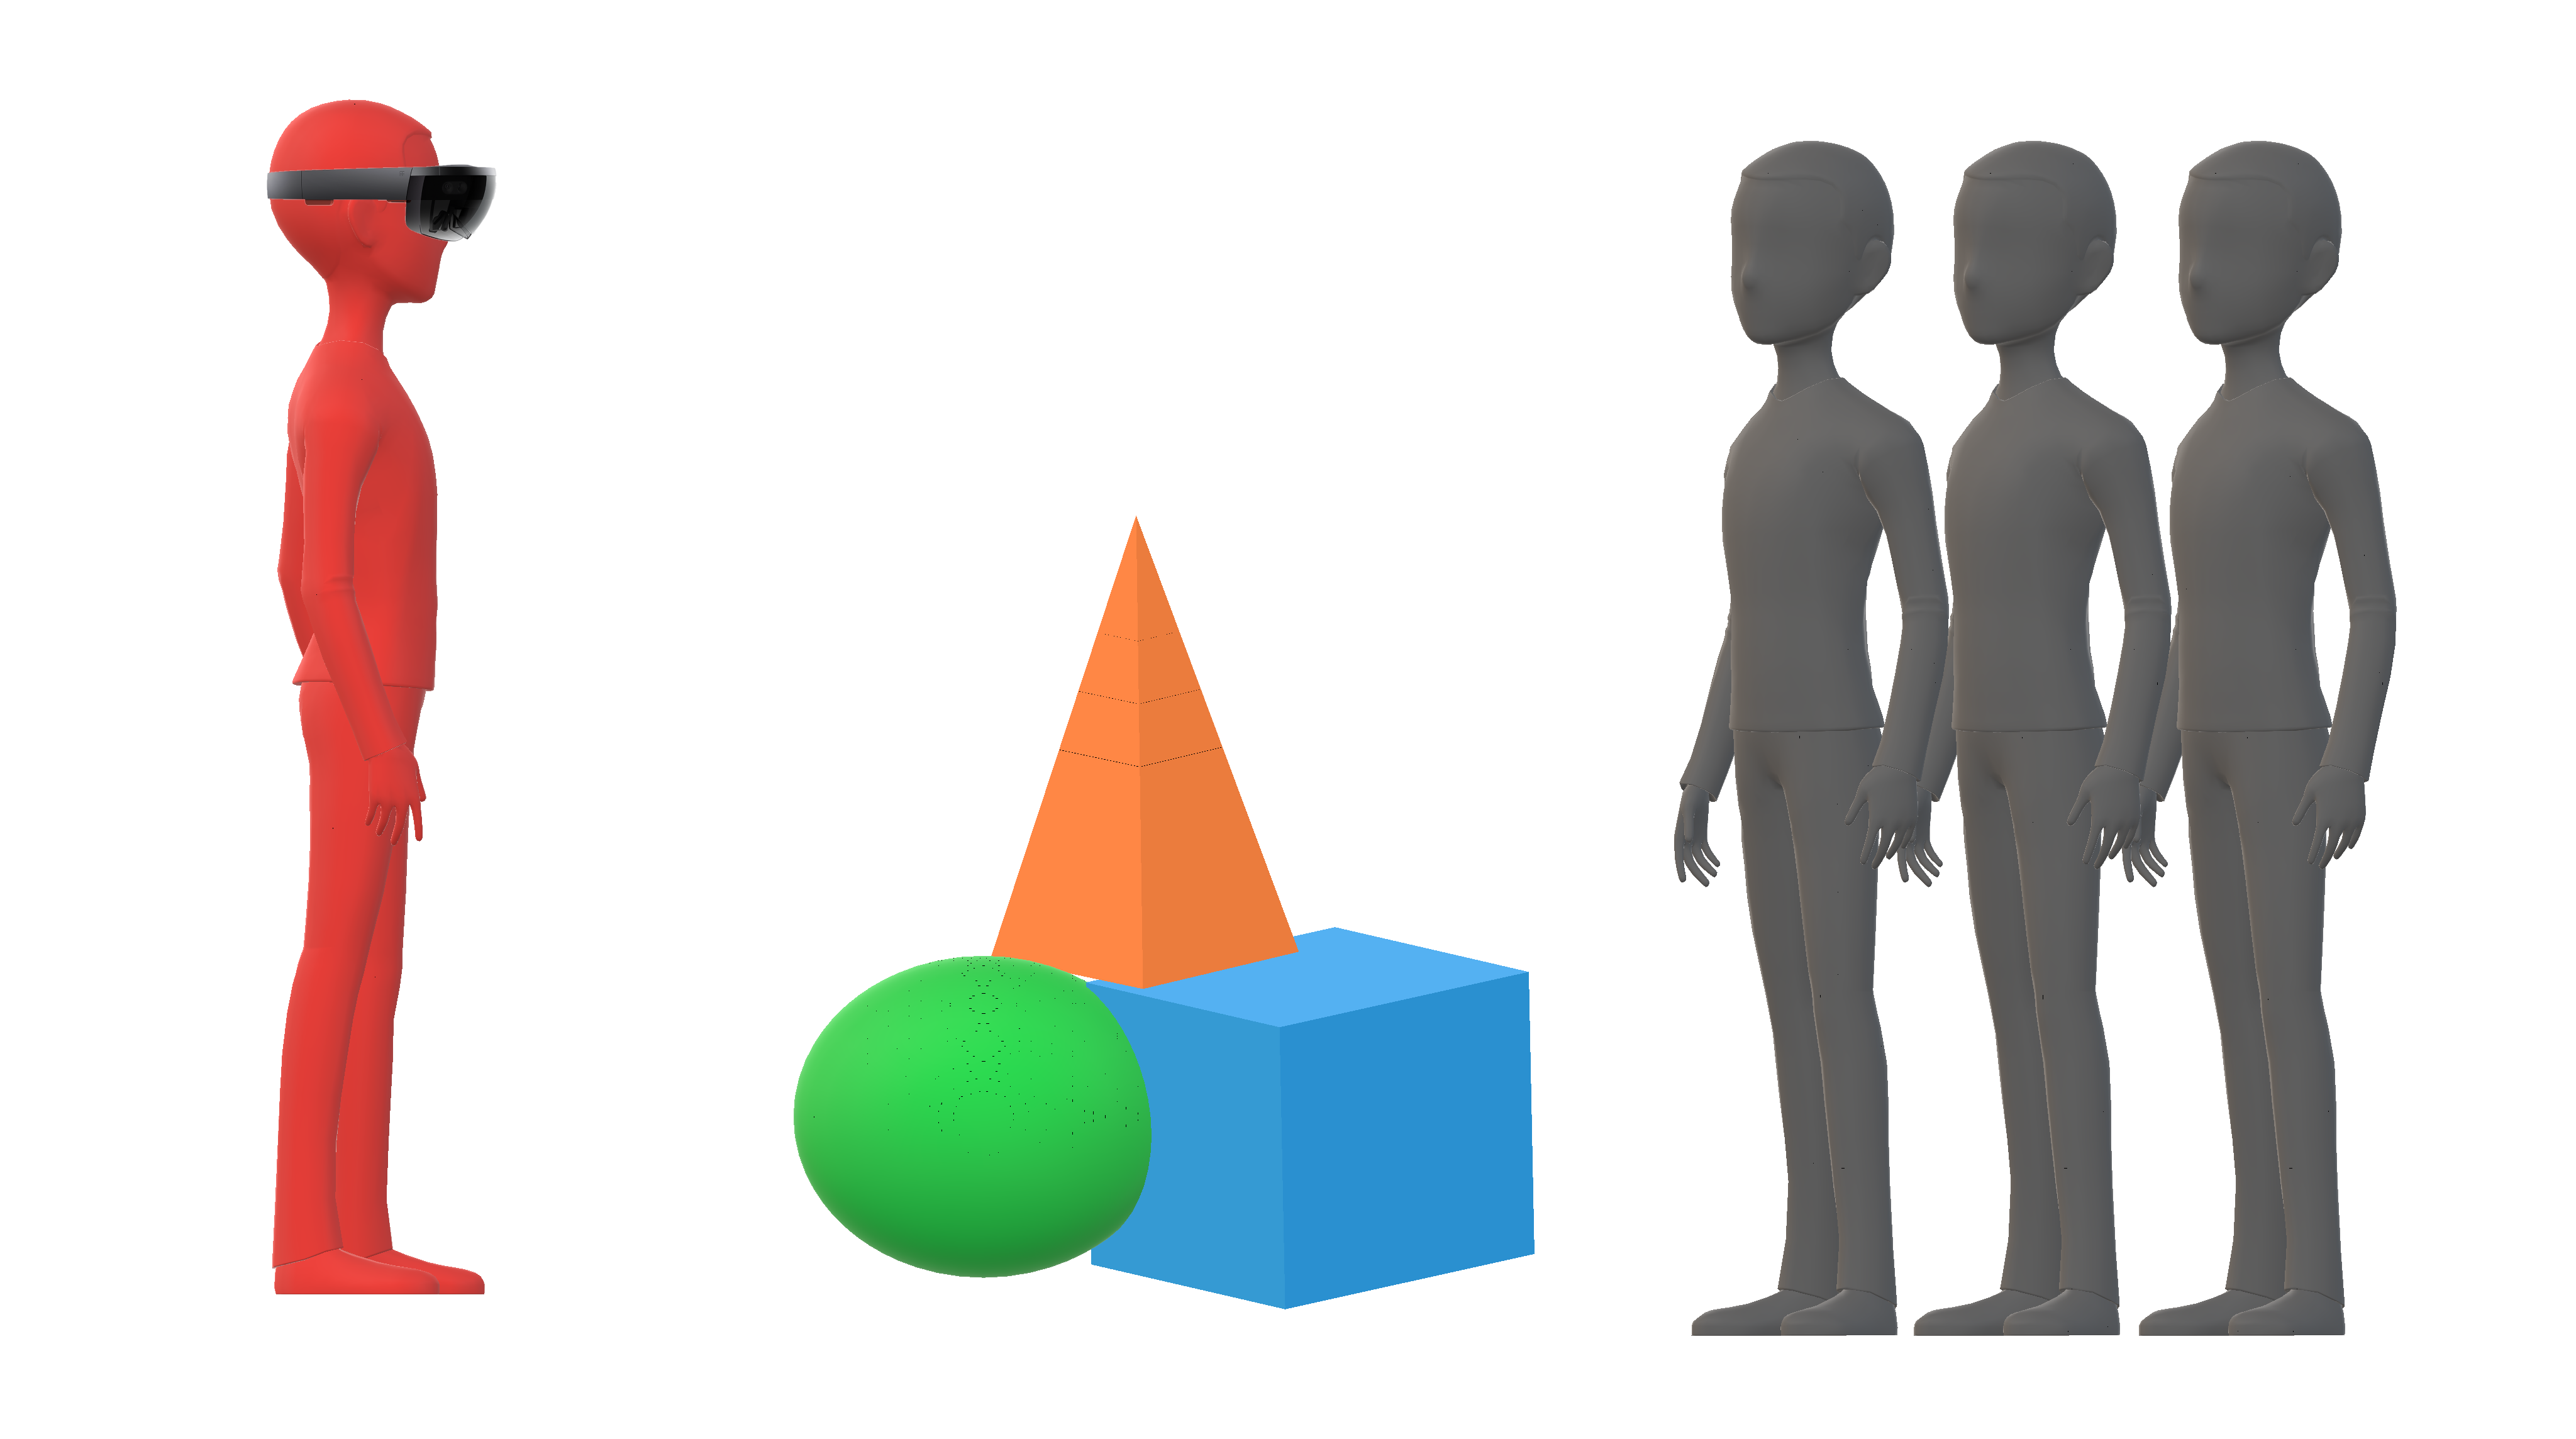
\includegraphics[width=3in]{images/continuum_categories5.png}
    \caption{The social AR continuum categories: 1) self and others, 2) objects and surrounding environments, 3) interaction and annotations}
    \label{fig:continuum:categories}
\end{figure}


% \section{Introduction}

% With wearable Augmented Reality (AR) devices becoming affordable, available and ubiquitous, there is a need to understand design considerations for this new platform. Previous research has looked into using AR headsets for collaborative use. The research presented here explores the use of AR headsets for social interaction and shared experiences. Social interactions can be extrapolated from current social network interactions where \enquote{friends} share content and interact with another's content (i.e., likes, comments).

% In the social AR/VR space, previous work implemented visual representations of self and others (e.g., Facebook Spaces\footnote{https://www.facebook.com/spaces}) to create fun overlays and representations of the face and upper body. In other research, \cite{Fanello2016} prototyped live sharing of a full scan of a person's body with remote users using 3D cameras and the HoloLens\footnote{https://www.microsoft.com/en-nz/hololens}. For representing “people” in AR space, \cite{Sousa2016} studied the concept of \enquote{personal space} and \enquote{social bubbles} in terms of proxemic interactions between people in different places. They used floor projections and hand-held devices to communicate the presence of remote people. They also established a \enquote{gradual engagement model for remote proxemic} based on distance from the user which consists of 1) personal, 2) engaged, 3) peripheral, and 4) ambient.

% Most work has focused on how visual representation and proximity could be used to organize an AR representation of a person's social network. However, this information could also be used to modify the contextual information being shared by a user out to their social network as well. For example, a person may not want strangers to know what they look like, and so would prefer being represented as a stylistic icon to people that do not know them, but would be more comfortable sharing a lifelike representation to those that are close to them. 
 
% In many mobile AR applications, the technology is used to share a view of the user's world. For example, remote expert collaboration systems have been developed where a local worker with an AR display can share a live video view of their workspace with a remote expert \cite{Billinghurst2002}. The remote expert can provide visual feedback with AR graphical cues.

% When people connect in this way, they may also want to share different amounts of information about their surroundings with each other. For example, users who are close in a social network may be happy to share a 3D virtual view of their surroundings and have the remote user appear as an AR avatar in their real space, while those that are strangers may only want to have an audio connection and not show anything of their surroundings to preserve their privacy but allow them to share and control their privacy \cite{Oetzel2011}. The position on the social continuum could be used to modify how much information a person can share about themselves and their surroundings.

This work aims to layout the space of the AR continuum for social sharing experiences by looking at parameters and options that can be changed in terms of people, objects and the environment to create a shared AR experience. This is still work in progress, but aims to cover all dimensions of the AR continuum.

\section{Social AR Continuum Dimensions}

As we established the social AR continuum varies based on the closeness of social connections that we have with others (relationship), we identified the following dimensions where social AR applications can fit along a continuum. The dimensions can be grouped in the categories described in Figure \ref{fig:continuum:dimensions}.

% \begin{figure}
%     \centering
%     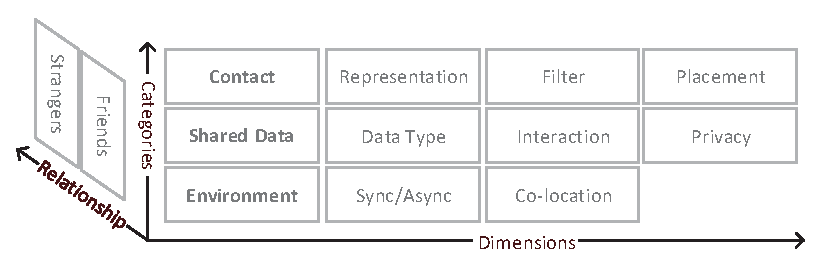
\includegraphics[width=3in]{images/dimensions-diagram-01.eps}
%     \caption{Dimensions of Social AR Continuum.}
%     \label{fig:continuum:dimensions}
% \end{figure}


\begin{figure}
    \centering
    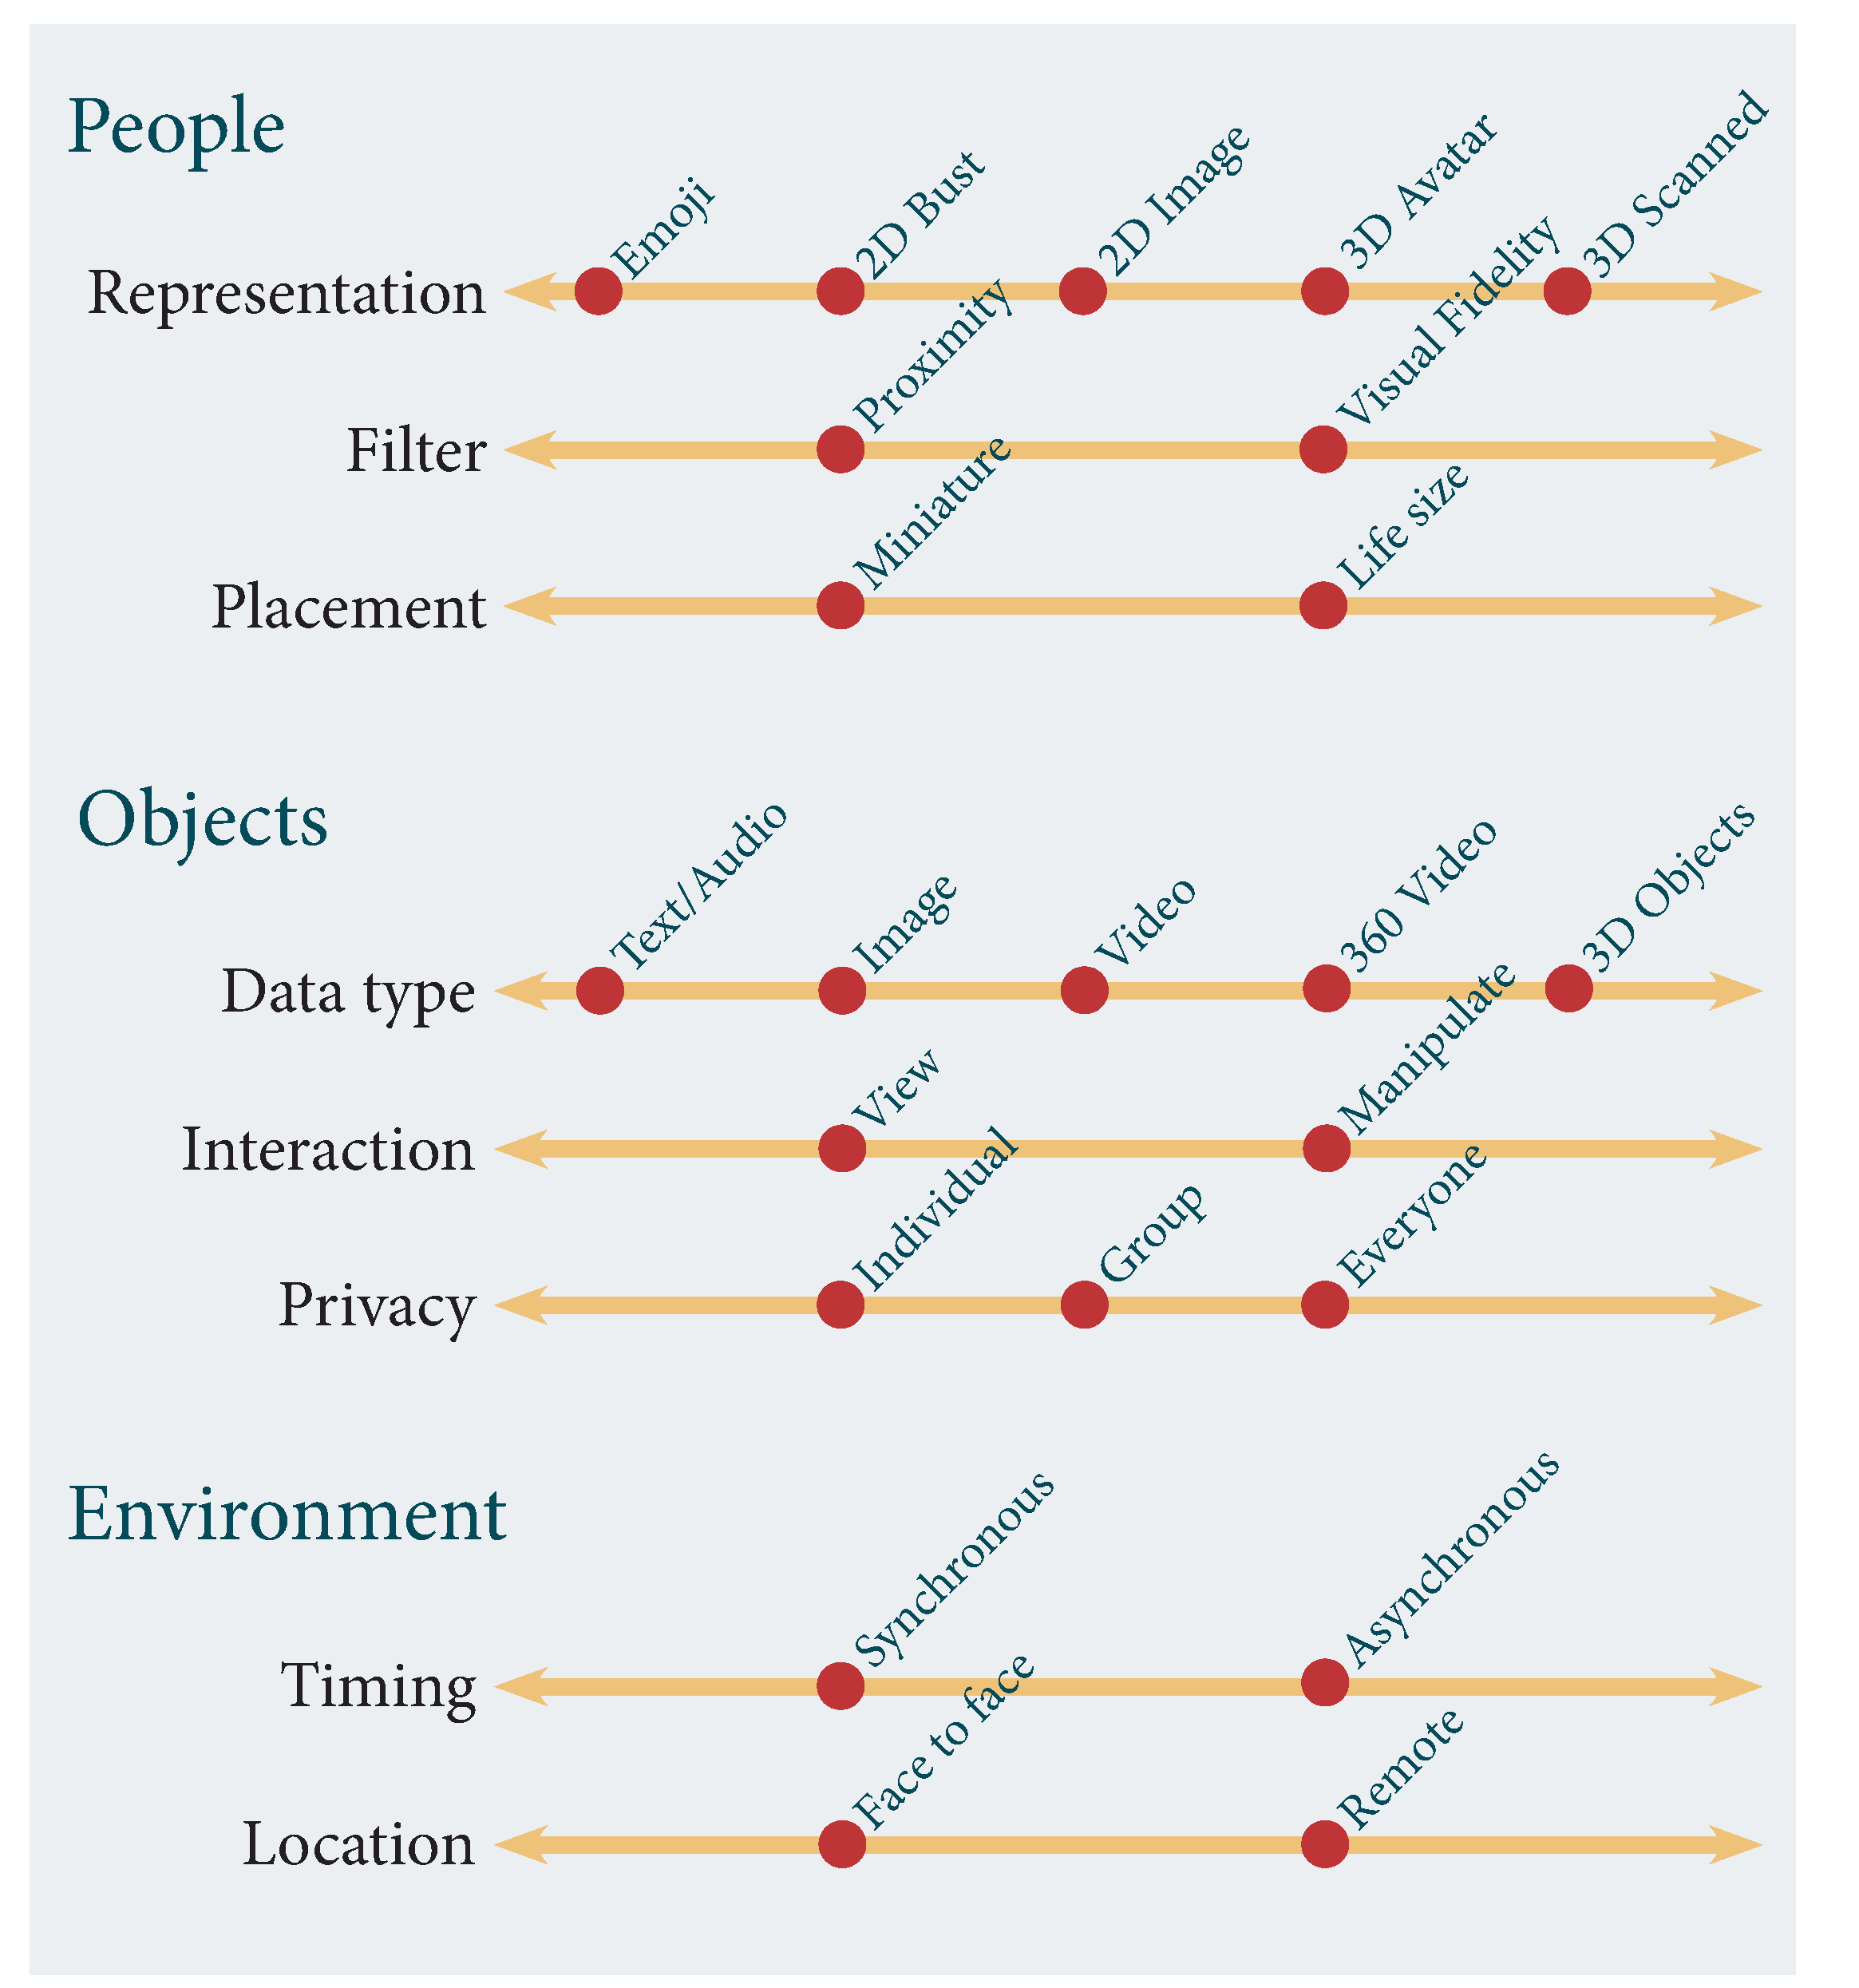
\includegraphics[width=3in]{images/continuum.eps}
    \caption{Dimensions of Social AR Continuum}
    \label{fig:continuum:dimensions}
\end{figure}

\textbf{Contact Representation}
Representing social contacts can vary on the social AR continuum based on the relationship that the user has with the contact. Intimate contacts can be represented as full 3D animated avatars. Friends could be represented as 2D static images, while Acquaintances could be represented as 2D busts, and strangers as merely emojis. Each contact could choose their own representation for each category.  

\textbf{Contact Filter}
Filtering social contacts to distinguish users from each other could be done using proximity or visual fidelity based on their relationship to the user. Proximity filters contacts by placing them closer or further-away. Visual fidelity filters contacts by adding more level of detail to the contact for closer relationships and less detail for further away contacts. 

\textbf{Contact Placement}
Placing social contacts can be done either by displaying them as life-size avatars on the ground around the user for close relationships, or by displaying them as miniatures on a distant surface. 

\textbf{Data Type}
The type of data shared between social contacts in AR can be categorised as 1D (e.g., text or audio), 2D (e.g., images, panorama or video), or 3D (e.g., 3D model or scanned-room environment). Based on the relationship between the user and his/her social contacts, the type of data available can be filtered. For instance, 3D data are shared with intimate relationships, while acquaintances can see only 2D data.  

\textbf{Data Interaction}
In terms of user interactions with shared data, the continuum here ranges from viewing the contents, annotating or adding comments on the content, through to manipulating the content. Levels of manipulation include changing the position, rotation or scale of the shared content, or even modifying the content itself

\textbf{Data Privacy}
Based on relationship with other users, shared data can be made private to the user, shared with specific groups of people (e.g., friends, acquaintances), or shared with everyone. 

\textbf{Sync/Async}
The data shared with contact can be shared in a synchronous way where both sharing and interaction happen at the same time. In contrast, data can be also shared asynchronously \cite{Smith2016} i.e., interaction happens at a different time. 

\textbf{Co-location}
Social contacts can either be remote (i.e., in a different place than the user) or face-to-face (i.e., physically in the same location as the user). When social contacts are remote, they are represented as virtual avatars based on their relationship with the user. An example of face-to-face interaction was described in a Black Mirror \footnote{http://www.imdb.com/title/tt2085059/} episode where a person could 'block' another co-located person by blurring them out in their AR view of the real world.

\section{Summary}

In this work, we introduced the concept of The Social AR Continuum. We identified several dimensions where a social AR application could be implemented. We created a prototype interface on one dimension -Contact Placement- comparing life-size to miniature avatars. From the collected data we found that both conditions were well received by potential users. In the future, we plan to explore other dimensions, study the effects of avatar realism, and report on users' perception of the continuum.
